\documentclass[a4paper,12pt,oneside,openany,table,xcdraw]{article}

\usepackage{setspace}
\usepackage{multirow}
\usepackage{hyperref}
\usepackage{caption}
\usepackage{indentfirst}
\usepackage{tikz} %% fasores
\usetikzlibrary{arrows,arrows.meta,quotes,angles}
\usepackage{siunitx}

\usepackage[brazilian]{babel}
\usepackage[utf8x]{inputenc}
\usepackage{amsmath, graphicx, subfig, enumerate}
\usepackage{float, verbatim}
\usepackage[colorinlistoftodos]{todonotes}
\usepackage{makeidx}
\usepackage{geometry}

\graphicspath{{img/}}
\geometry{a4paper, hmargin={3cm, 3cm}, vmargin={3cm, 2cm} }
\setlength{\parindent}{1.0cm}
\captionsetup{font=small}

\usepackage{mathtools,listings} %%
\usepackage{color} %red, green, blue, yellow, cyan, magenta, black, white
\definecolor{mygreen}{RGB}{28,172,0} % color values Red, Green, Blue
\definecolor{mylilas}{RGB}{170,55,241}
\usepackage{listingsutf8}

\begin{document}
\newcommand{\thedepartment}{Faculdade de Engenharia Elétrica}
\newcommand{\thecourse}{FEELT}
\newcommand{\thetitle}{Resolução da Lista de Exercícios 1}
\newcommand{\thetype}{Trabalho de Princípios de Comunição}
\newcommand{\theproftitle}{Bacharel em Engenharia Elétrica}
\newcommand{\thestudent}{Lesly Viviane Montúfar Berrios\\
\centering11811ETE001}
\newcommand{\theadvisor}{Prof. Lorenço Santos Vasconcelos}
\newcommand{\thecity}{Uberlândia}

\thispagestyle{empty}\newcommand*{\themonth}{\ifthenelse{\the\month < 2}{Janeiro }
                  {\ifthenelse{\the\month < 3}{Fevereiro }
                  {\ifthenelse{\the\month < 4}{Março }
                  {\ifthenelse{\the\month < 5}{Abril }
                  {\ifthenelse{\the\month < 6}{Maio }
                  {\ifthenelse{\the\month < 7}{Junho }
                  {\ifthenelse{\the\month < 8}{Julho }
                  {\ifthenelse{\the\month < 9}{Agosto }
                  {\ifthenelse{\the\month < 10}{Setembro }
                  {\ifthenelse{\the\month < 11}{Outubro }
                  {\ifthenelse{\the\month < 12}{Novembro }{Dezembro }}}}}}}}}}}}
                  
\begin{titlepage}
\begin{center}

	\vspace{-0.5cm}

  \begin{figure}[hbt!]
		\begin{center}
		   
\includegraphics[width=2.8cm]{ufu-logo.png}
		\end{center}
	\end{figure}
 	%\vspace{-4cm}

%\begin{doublespacing}

  \Large{\textbf{Universidade Federal de Uberlândia}}\\
  \large{\thedepartment}\\
  \large{\thecourse}\\


\vspace{5.8cm}
  \par
  \large\textbf{\thetitle}
\vspace{5.8cm} 

%\end{doublespacing}
  \par
  \thetype\\
  por\\
  %\hspace{2cm}\large{}\\

\vspace{0.8cm}
\par
  \normalsize{\thestudent}\\ [2cm]
  \theadvisor

\par\vfill
  \thecity, \themonth / \the\year

\end{center}

\end{titlepage}

\lstset{language=Matlab,%
	inputencoding=utf8/latin1,
    %basicstyle=\color{red},
    breaklines=true,%
    morekeywords={matlab2tikz},
    keywordstyle=\color{blue},%
    morekeywords=[2]{1}, keywordstyle=[2]{\color{black}},
    identifierstyle=\color{black},%
    stringstyle=\color{mylilas},
    commentstyle=\color{mygreen},%
    showstringspaces=false,%without this there will be a symbol in the places where there is a space
    numbers=left,%
    numberstyle={\tiny \color{black}},% size of the numbers
    numbersep=9pt, % this defines how far the numbers are from the text
    emph=[1]{for,end,break},emphstyle=[1]\color{red}, %some words to emphasise
    %emph=[2]{word1,word2}, emphstyle=[2]{style},    
}

%% Comeca o documento !

\onehalfspacing
\tableofcontents % sumário
\newpage

\section{Exercício 1}
O gráfico correspondente aos Sinais Básicos Importantes é mostrado na Figura \ref{ex1:figure} e o código que a gerou no Anexo \ref{anexo:ex1}.

\vspace{0.4cm}
\begin{figure}[H]
\centering
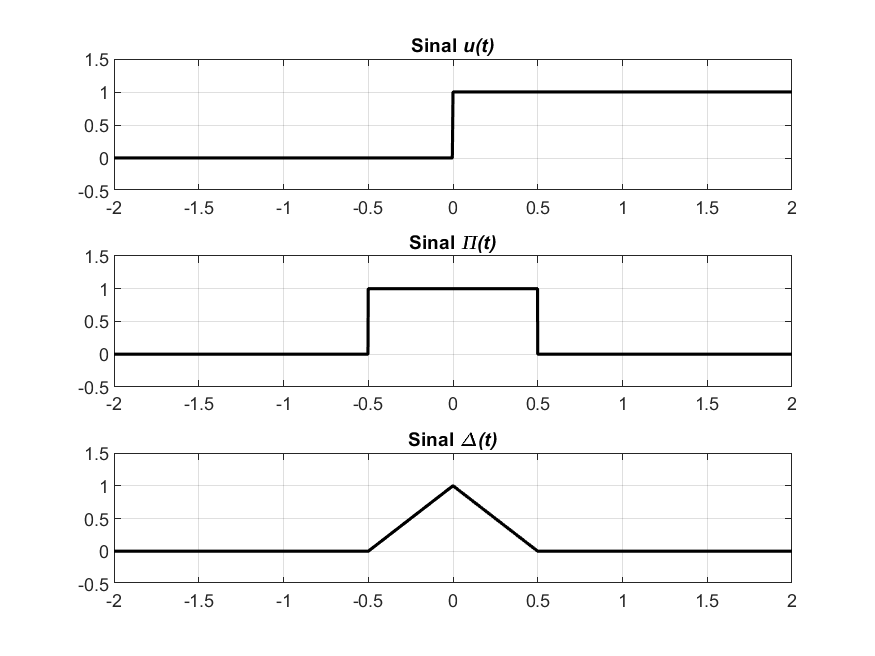
\includegraphics[width=16cm]{ex1-fig}
\caption{Sinais Básicos Importantes.}
\label{ex1:figure}
\end{figure}

\vspace{0.3cm}
\section{Exercício 2}
A seguir nas Figuras \ref{ex2:separado} e \ref{ex2:mult}, tem-se os gráficos referentes aos sinais separados e depois multiplicados respectivamente.

\vspace{0.4cm}
\begin{figure}[H]
\centering
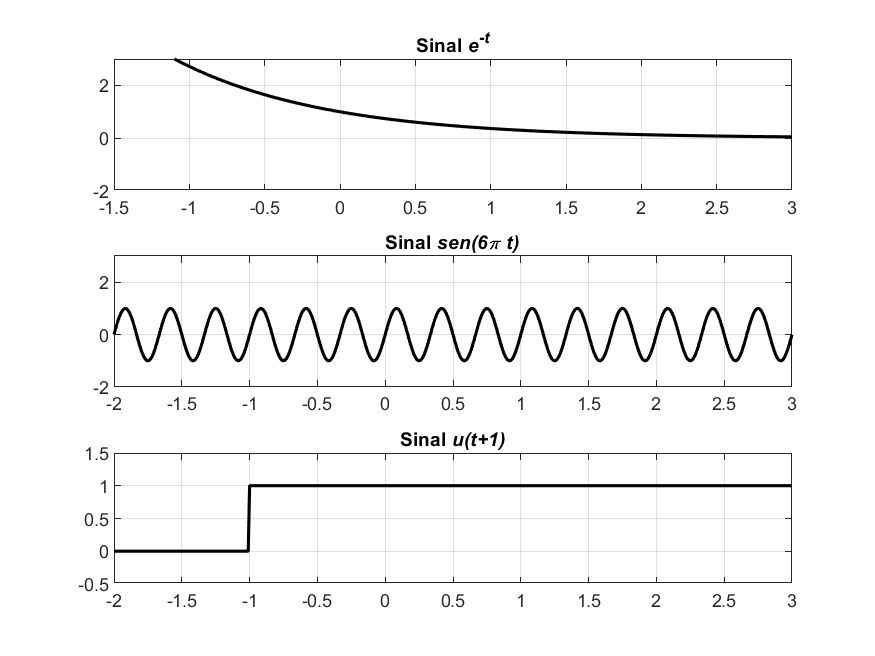
\includegraphics[width=14cm]{ex2-separado}
\caption{Sinais separados.}
\label{ex2:separado}
\end{figure}

\vspace{0.4cm}
\begin{figure}[H]
\centering
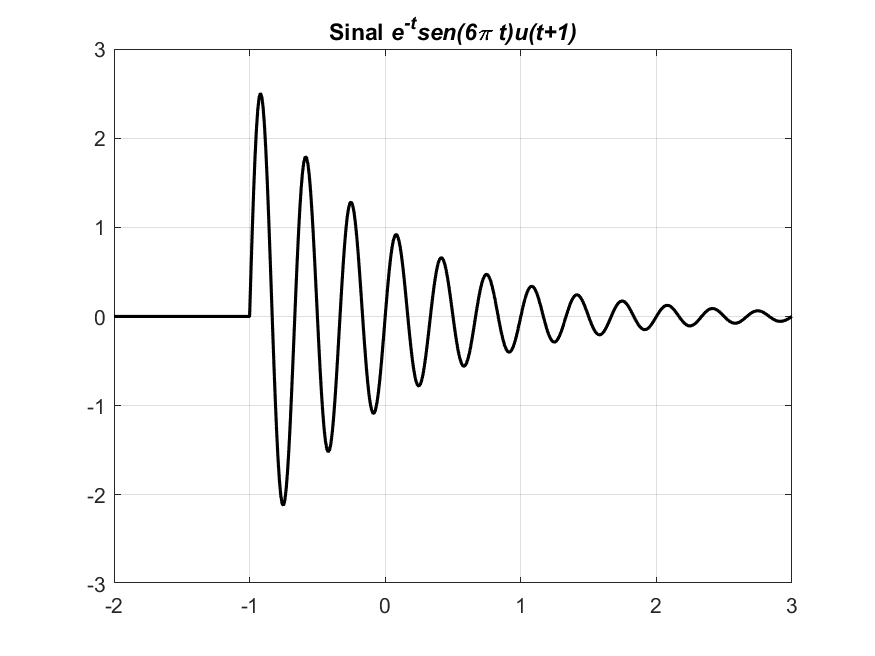
\includegraphics[width=14cm]{ex2-mult}
\caption{Sinais multiplicados.}
\label{ex2:mult}
\end{figure}

\vspace{0.3cm}
\section{Exercício 3}
Dado um sinal aperiódico, sua repetição gera um sinal periódico como o da Figura \ref{ex3:sinal}. Além disso, é possível extrair dados como a \textit{Energia = 48,7753 J} e \textit{Potência = 8,12922 W}. O Anexo \ref{anexo:ex3} comtempla o código utilizado neste exercício.

\vspace{0.4cm}
\begin{figure}[H]
\centering
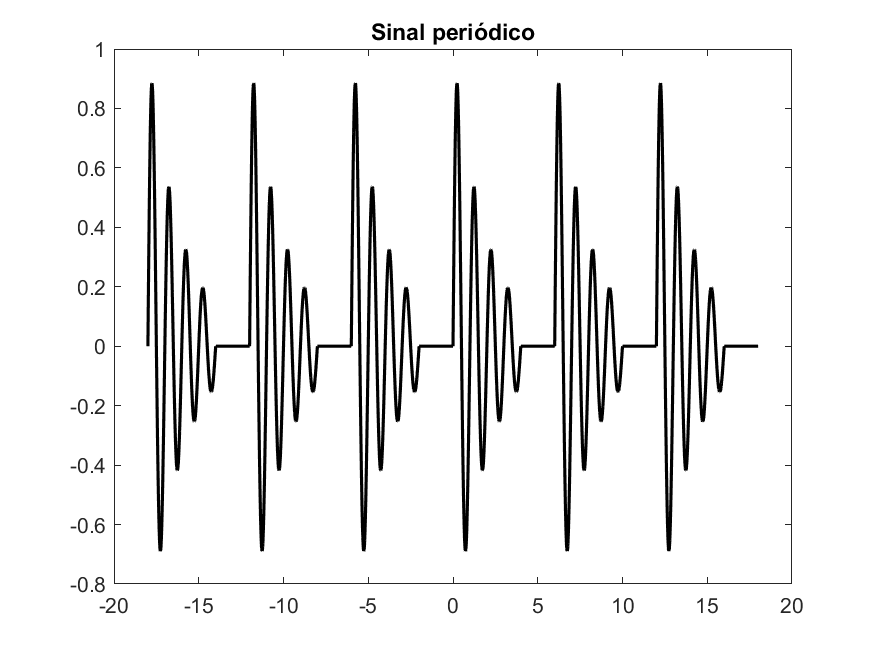
\includegraphics[width=16cm]{ex3-sinal}
\caption{Sinal periódico.}
\label{ex3:sinal}
\end{figure}

\vspace{0.3cm}
\section{Exercício 4}
O coeficiente de correlação entre a função $x(t)$ e $g_i(t)$, descrito como na Equação \ref{corr}, para cada função $g$, é comtemplado na Figura \ref{ex4:corr}. No Anexo \ref{anexo:ex3} observa-se o código utilizado neste exercício.

\vspace{0.4cm}
\begin{equation} \label{corr}
\rho = \dfrac{1}{\sqrt{E_g\ E_x}} \int^{+\infty} _{-\infty} {g(t)\ x^*(t)} dt
\end{equation}

\vspace{0.4cm}
\begin{figure}[H]
\centering
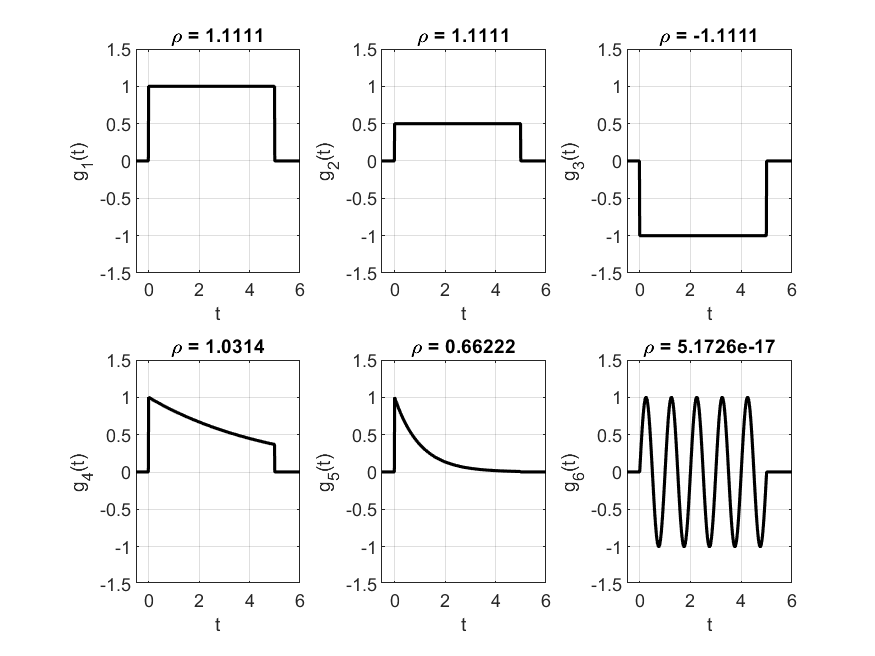
\includegraphics[width=16cm]{ex4-corr}
\caption{Correlação de sinais.}
\label{ex4:corr}
\end{figure}
 
\newpage
\section{Anexos}
\subsection{Código correspondente ao exercício 1} \label{anexo:ex1}
\lstinputlisting{Code/EX1.m}
\vspace{0.3cm}

\lstinputlisting{Code/u.m}
\vspace{0.3cm}

\lstinputlisting{Code/rect.m}
\vspace{0.3cm}

\lstinputlisting{Code/Delta.m}

\vspace{0.3cm}
\subsection{Código correspondente ao exercício 2} \label{anexo:ex2}
\lstinputlisting{Code/EX2.m}

\vspace{0.3cm}
\subsection{Código correspondente ao exercício 3} \label{anexo:ex3}
\lstinputlisting{Code/EX3.m}
\vspace{0.3cm}

\lstinputlisting{Code/energia.m}

\vspace{0.3cm}
\subsection{Código correspondente ao exercício 4} \label{anexo:ex4}
\lstinputlisting{Code/EX4.m}
\vspace{0.3cm}

\lstinputlisting{Code/correlacao.m}

\newpage
\begin{thebibliography}{9} 
% Introdução
%\bibitem{S1}
%    Gene F. Franklin, J. David Powell, Abbas Emami-Naieni.,
%    “Sistemas de Controle para a Engenharia”, Porto Alegre: Bookman, 2013.

%\bibitem{S2}
%    Oppeinheim, Alan V.; Willsky, Allan S.,
%    “Sinais e Sistemas”, São Paulo: Pearson
%Prentice Hall, 2010. 2ª Edição.

\bibitem{S2}
    Lathi, B. P.; Ding, Zhi,
    “Modern Digital and Analog Communication Systems”, New York: 
    Oxford University Press, 2019. 5ª Edição.

\end{thebibliography}
\end{document}
